\subsectionA{B'rohg}
B'rohgs are a species of four-armed humanoids akin to giants. Simpleminded, nomadic hunters and gatherers, b'rohgs tend to keep to themselves, only attacking when they feel threatened. Bands have been known to turn to raiding in desperate situations. B'rohgs are often captured and put to work in the arena as gladiators. Some are even tricked into service with promises of food and sweetmeats but this is the exception rather than the rule. Most b'rohgs are not intelligent enough to remember their friends, let alone long-term promises.

Although they are treated like animals by their owners, enslaved b'rohgs still possess enough cunning to be able to escape from time to time. These ``renegade'' b'rohgs often have developed considerable skill with weaponry and combat techniques during their time in captivity and are viewed with concern as a result b'rohgs communicate through a series of grunts and hand signals. Adult b'rohgs stand about 5 meters high.

\subsubsection{B'rohg Society}
Dominated by their strongest males, b'rohgs are a throwback to simpler times. They live in small nomadic bands comprised of 1--4 family units called cliques, consisting of one male, one or two females, and generally fewer than four total offspring. The strongest b'rohg in a band will primarily be hunters, while the older, weaker members and the children are gatherers and water bearers.
\begin{figure}[t!]
\centering
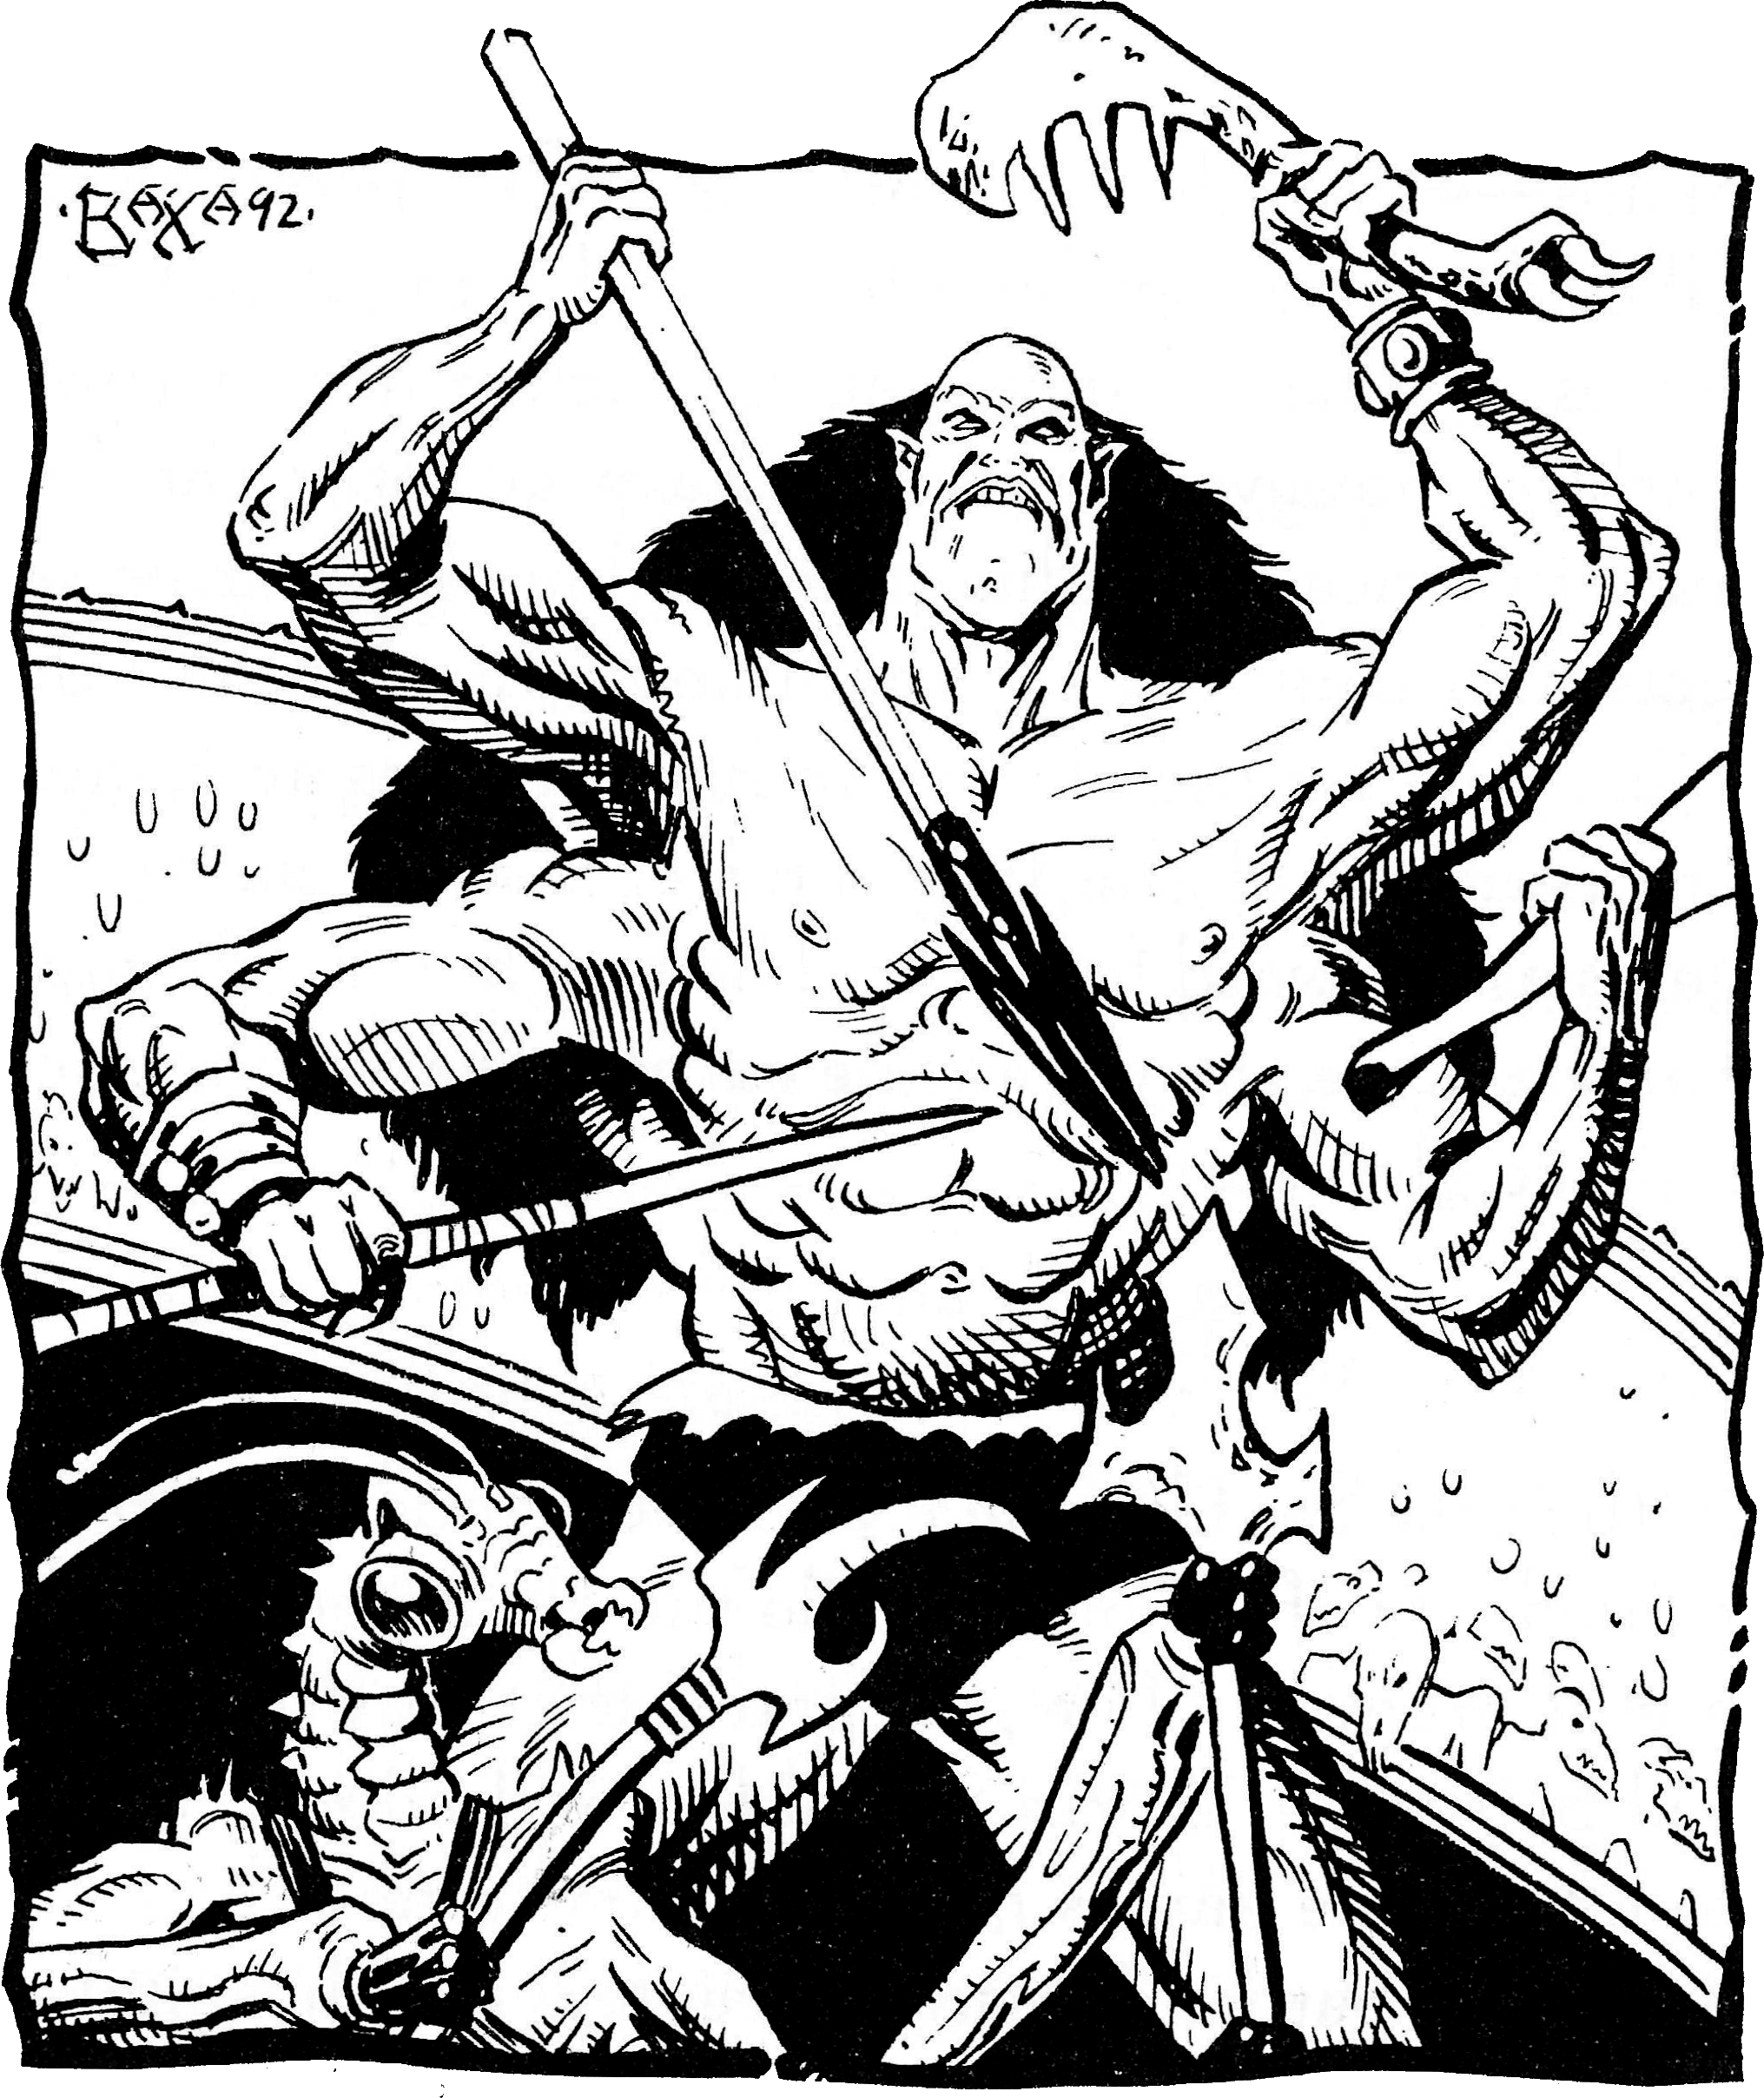
\includegraphics[width=\columnwidth]{images/b-rohg-2.png}
\WOTC
\end{figure}

B'rohgs have no mastery of fire but do not fear it. They also have no real understanding of death and will ignore objects or creatures that do not display signs of life (although they have learned that ``playing dead'' is a tactic sometimes used by their foes and will repeatedly strike felled enemies, just to be sure).

While they are too stupid to learn more contemporary speech, others can learn the grunt and sign language of the b'rohgs.

\subsubsection{B'rohg Racial Traits}
\begin{itemize*}
    \item +14 Strength, +4 Dexterity, +8 Constitution, $-6$ Intelligence: B'rohgs are stupid but very strong and agile.
    \item Huge: $-2$ penalty to Armor Class, $-2$ penalty on attack rolls, $-8$ penalty on \skill{Hide} checks, +8 bonus on grapple checks, lifting and carrying limits quadruple those of Medium characters.
    \item B'rohgs occupy a space of 4.5 meters and have a reach of 4.5 meters.
    \item Giant: B'rohgs are creatures with the giant type.
    \item B'rohg base land speed is 12 meters. B'rohg base climb speed is 6 meters. B'rohg have +8 racial bonus on \skill{Climb} checks. They can always choose to take 10 on a \skill{Climb} check, even if rushed or threatened.
    \item Low-light vision: B'rohgs can see twice as far as a human in moonlight and similar conditions of poor illumination, retaining the ability to distinguish color and detail.
    \item Racial Hit Dice: A b'rohg begins with 6 levels of giant, which provide 6d8 Hit Dice, a base attack bonus of +4, and base saving throw bonuses of Fort +5, Ref +2 and  Will +2.
    \item Racial Skills: A b'rohg's giant levels give it skill points equal to 9 $\times$ (2 + Int modifier). Its class skills are \skill{Climb}, \skill{Listen}, \skill{Spot} and \skill{Survival}.
    \item Racial Feats: A b'rohg's giant levels give it 3 feats.
    \item Weapon Proficiency: A b'rohg is proficient with simple and martial weapons as well as its natural weaponry.
    \item Natural Armor: +6 natural armor bonus to AC.
    \item Natural Weapons: 4 slams (1d6).
    \item Rock Catching (Ex): Once per round, a b'rohg that would normally be hit by a rock can make a Reflex save to catch a rock (or similar projectile) as a free action. The DC is 15 for a Small rock, 20 for a Medium one, and 25 for a Large one (if the projectile provides a magical bonus on attack rolls, the DC increases by that amount.) The b'rohg must be ready for and aware of the attack in order to make a rock catching attempt.
    \item Rock Throwing (Ex): Adult b'rohgs are accomplished rock throwers and receive a +1 racial bonus on attack rolls when throwing rocks. A b'rohg of at least Huge size can hurl rocks weighing 30 to 40 kilograms each (Medium objects) up to five range increments. The size of the range increment is 42 meters.
    \item Automatic Languages: B'rohg. Bonus Languages: none.
    \item Favored Class: Ranger.
    \item Level Adjustment: +6.
\end{itemize*}
